%GiG
\documentclass{beamer} 
\usetheme{Copenhagen}
\setbeamertemplate{navigation symbols}{}
\setbeamertemplate{headline}{}
\DeclareMathOperator*{\argmax}{arg\,max}

\usepackage{hyperref}


\definecolor{azure}{rgb}{0.0, 0.5, 1.0}
%\newcommand{\tblue}[1]{\textcolor{blue}{#1}}
\newcommand{\tblue}[1]{{\Large {\textcolor{azure}{#1}}}}
\newcommand{\thblue}[1]{{\Huge {\textcolor{azure}{#1}}}}
\newcommand{\hred}[1]{{\textcolor{red}{#1}}}
\newcommand{\furl}[1]{{\footnote{\url{#1}}}}

\newcommand{\mypause}{\pause}
%\newcommand{\mypause}{}

\title[Saravanan Thirumuruganathan] 
{Lecture 7: Decision Trees}

\author[CSE 5334] 
{Instructor: Saravanan Thirumuruganathan}

\date[] 

\begin{document}


\begin{frame}
  \titlepage
\end{frame}

%\begin{frame}{Outline}
%  \tableofcontents
%  % You might wish to add the option [pausesections]
%\end{frame}

\section{Outline}

\begin{frame}
\frametitle {Outline}
\begin{enumerate}
\item Geometric Perspective of Classification
\item Decision Trees
\end{enumerate}
\end{frame}


%\begin{frame}{In-Class Quizzes}
%\begin{itemize}
%\item {\Large {\bf URL:}} {\LARGE \bf \url{http://m.socrative.com/}} 
%\item {\Large {\bf Room Name:} {\LARGE \bf 4f2bb99e}}
%\end{itemize}
%\end{frame}


\section{Geometric Perspective of Classification}
\begin{frame}{} 
    \begin{center}
        \thblue{Geometric Perspective of Classification}
    \end{center}
\end{frame}

\begin{frame}{Perspective of Classification}
    \begin{itemize}
        \item Algorithmic
        \item Geometric 
        \item Probabilistic
        \item $\ldots$
    \end{itemize}
\end{frame}

\begin{frame}{Geometric Perspective of Classification}
    \begin{itemize}
        \item Gives some intuition for model selection
        \item Understand the distribution of data
        \item Understand the expressiveness and limitations of various classifiers
    \end{itemize}
\end{frame}

\begin{frame}{Feature Space\footnote{DMA Book}}
    \begin{center}
        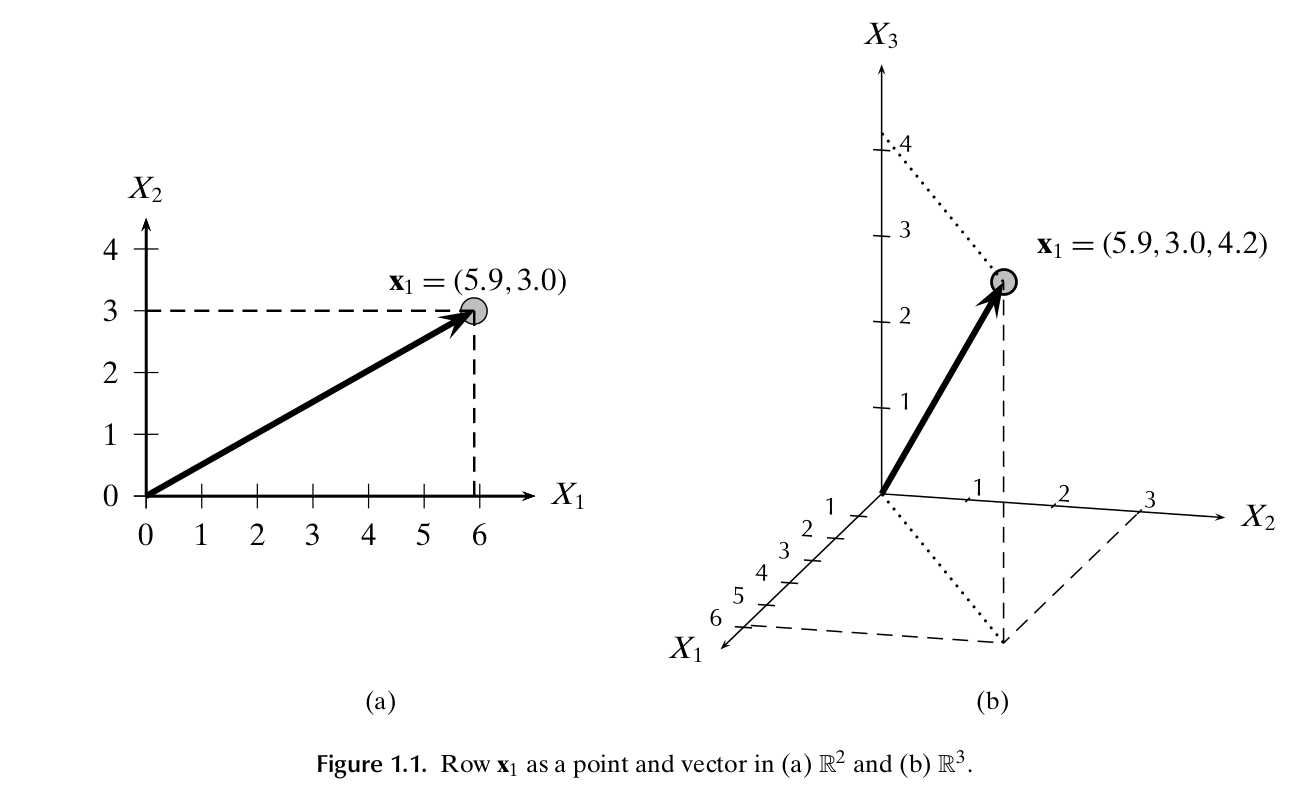
\includegraphics[scale=0.15]{geometricView.png}
    \end{center}
    \begin{itemize}
        \item {\bf Feature Vector:} $d$-dimensional vector of features describing the object
        \item {\bf Feature Space:} The vector space associated with feature vectors
    \end{itemize}
\end{frame}

\begin{frame}{Feature Space in Classification}
    \begin{center}
        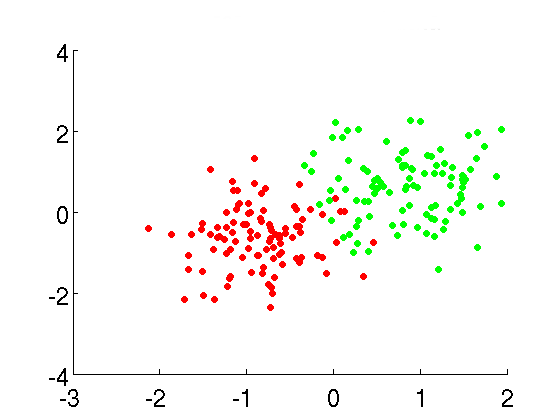
\includegraphics[scale=0.5]{featureSpace.png}
    \end{center}
\end{frame}

\begin{frame}{Geometric Perspective of Classification}
    \begin{itemize}
        \item {\bf Decision Region:} A partition of feature space such that all feature vectors in it are assigned to same class.
        \item {\bf Decision Boundary:} Boundaries between neighboring decision regions
    \end{itemize}
\end{frame}


\begin{frame}{Geometric Perspective of Classification}
    \begin{itemize}
        \item Objective of a classifier is to {\em approximate} the ``real'' decision boundary as much as possible 
        \item Most classification algorithm has specific expressiveness and limitations
        \item If they align, then classifier does a good approximation
    \end{itemize}
\end{frame}

\begin{frame}{Linear Decision Boundary}
    \begin{center}
        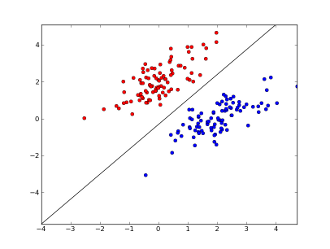
\includegraphics[scale=0.75]{linearDecisionBoundary.png}
    \end{center}
\end{frame}
\begin{frame}{Piecewise Linear Decision Boundary\footnote{ISLR Book}}
    \begin{center}
        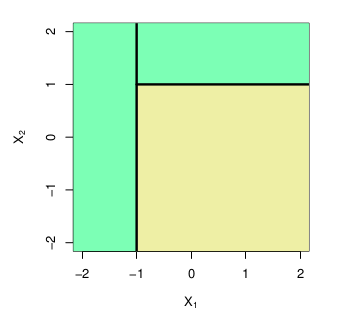
\includegraphics[scale=0.6]{piecewiseLinearDecisionBoundary.png}
    \end{center}
\end{frame}
\begin{frame}{Quadratic Decision Boundary\footnote{Figshare.com}}
    \begin{center}
        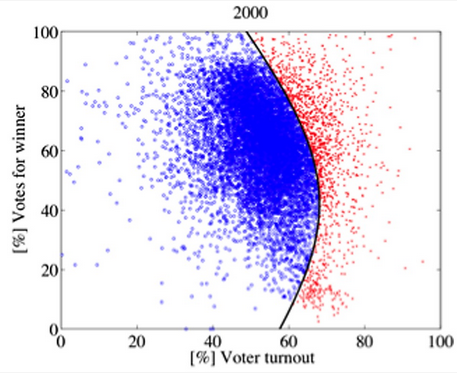
\includegraphics[scale=0.5]{quadraticDecisionBoundary.png}
    \end{center}
\end{frame}
\begin{frame}{Non-linear Decision Boundary\footnote{ISLR Book}}
    \begin{center}
        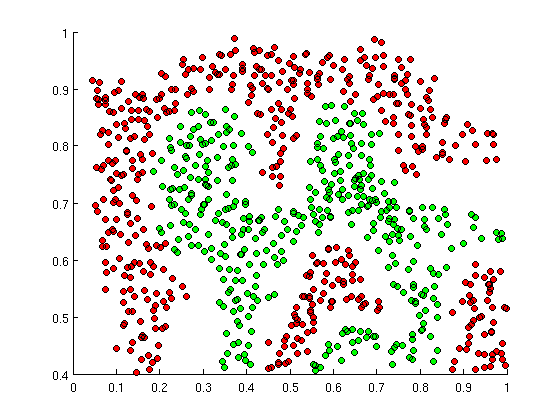
\includegraphics[scale=0.5]{nonlinearDecisionBoundary.png}
    \end{center}
\end{frame}
\begin{frame}{Complex Decision Boundary\footnote{ISLR Book}}
    \begin{center}
        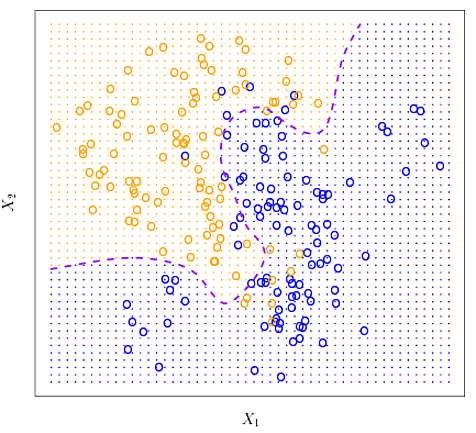
\includegraphics[scale=0.5]{complexDecisionBoundary.png}
    \end{center}
\end{frame}

\begin{frame}{Classifier Selection Tips}
    \begin{itemize}
        \item If decision boundary is linear, most {\em linear} classifiers will do well
        \item If decision boundary is non-linear, we sometimes have to use kernels 
        \item If decision boundary is piece-wise, decision trees can do well
        \item If decision boundary is too complex, $k$-NN might be a good choice
    \end{itemize}
\end{frame}

\begin{frame}{$k$-NN Decision Boundary\footnote{ISLR Book}}
    \begin{center}
        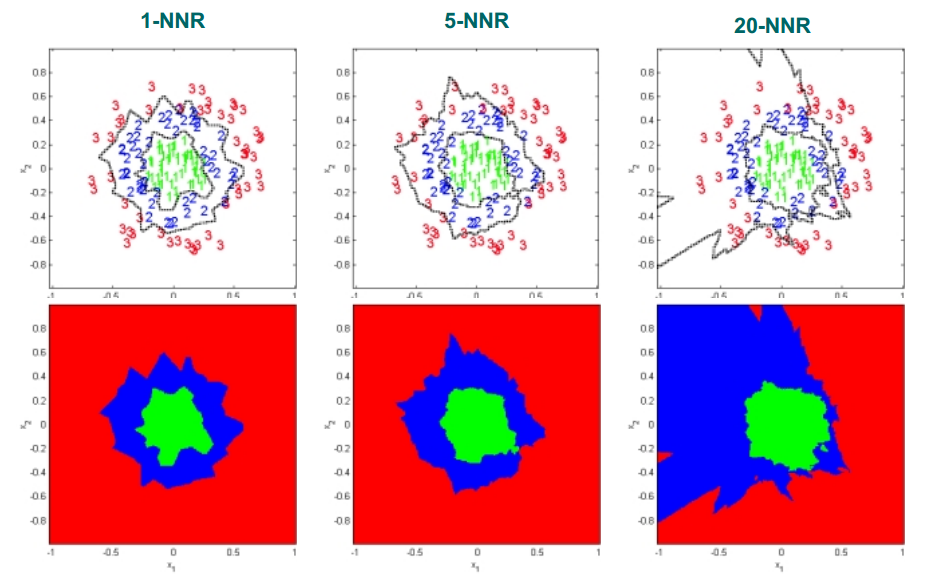
\includegraphics[scale=0.2]{kNNVaringK.png}
    \end{center}

    \begin{itemize}
       \item Asymptotically Consistent: With infinite training data and large enough $k$, $k$-NN approaches the best possible classifier (Bayes Optimal)
       \item With infinite training data and large enough $k$, $k$-NN could approximate most possible decision boundaries
    \end{itemize}
\end{frame}

\section{Decision Trees}
\begin{frame}{} 
    \begin{center}
        \thblue{Decision Trees}
    \end{center}
\end{frame}

\begin{frame}{Strategies for Classifiers}
    \begin{itemize}
        \item {\bf Parametric Models: } Makes some assumption about data distribution such as density and often use explicit probability models
        \item {\bf Non-parametric Models: } No prior assumption of data and determine decision boundaries directly.
        \begin{itemize}
            \item $k$-NN
            \item Decision tree
        \end{itemize}
    \end{itemize}
\end{frame}

\begin{frame}{Tree\furl{http://statweb.stanford.edu/~lpekelis/talks/13_datafest_cart_talk.pdf}}
    \begin{center}
        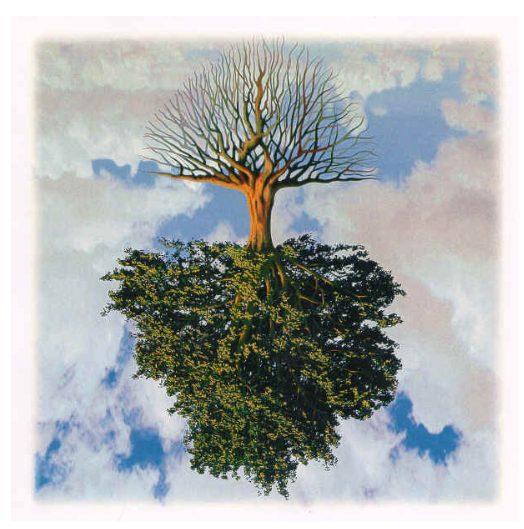
\includegraphics[scale=0.4]{tree.png}
    \end{center}
\end{frame}
\begin{frame}{Binary Decision Tree\furl{http://statweb.stanford.edu/~lpekelis/talks/13_datafest_cart_talk.pdf}}
    \begin{center}
        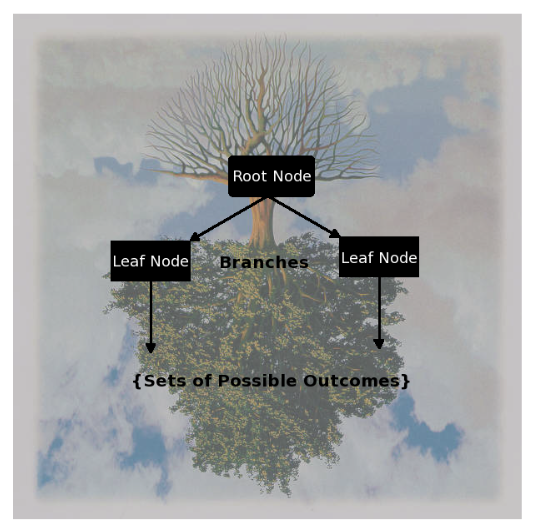
\includegraphics[scale=0.4]{binaryDTree.png}
    \end{center}
\end{frame}
\begin{frame}{20 Question Intuition\furl{http://www.idiap.ch/~fleuret/files/EE613/EE613-slides-6.pdf}}
    \begin{center}
        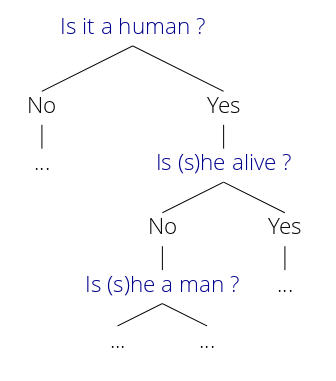
\includegraphics[scale=0.4]{20QAsDTree.png}
    \end{center}
\end{frame}
\begin{frame}{Decision Tree for Selfie Stick\footnote{The Oatmeal Comics}}
    \begin{center}
        
\includegraphics[scale=0.30]{selfie_stick.jpg}
    \end{center}
\end{frame}

\begin{frame}{Decision Trees and Rules\furl{http://artint.info/slides/ch07/lect3.pdf}}
    \begin{center}
        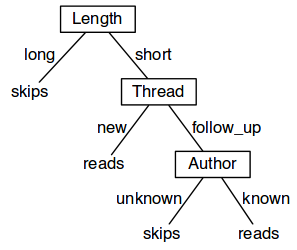
\includegraphics[scale=0.50]{egDTrees.png}
    \end{center}
\end{frame}
\begin{frame}{Decision Trees and Rules\furl{http://artint.info/slides/ch07/lect3.pdf}}
    \begin{columns}
        \column{0.58\linewidth}
            \begin{itemize}
                \item long $\rightarrow$ skips
                \item short $\wedge$ new $\rightarrow$ reads 
                \item short $\wedge$ follow Up $\wedge$ known $\rightarrow$ reads 
                \item short $\wedge$ follow Up $\wedge$ unknown $\rightarrow$ skips 
            \end{itemize}
            
        \column{0.38\linewidth}
            \centering
            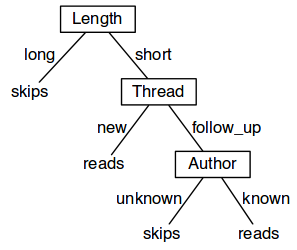
\includegraphics[scale=0.40]{egDTrees.png}
    \end{columns}
\end{frame}

\begin{frame}{Building Decision Trees Intuition\furl{http://spark-summit.org/wp-content/uploads/2014/07/Scalable-Distributed-Decision-Trees-in-Spark-Made-Das-Sparks-Talwalkar.pdf}}
\begin{center}
    \begin{table}
        \begin{tabular}{| c | c | c |}
            \hline
            {\bf Horsepower} & {\bf Weight} & \textcolor{blue}{{\bf Mileage}} \\ \hline
                95 & low & low \\ \hline
                90 & low & low \\ \hline
                70 & low & high \\ \hline
                86 & low & high \\ \hline
                76 & high & low \\ \hline
                88 & high & low \\ \hline
        \end{tabular}
        \caption{Car Mileage Prediction from 1971}
    \end{table}
\end{center}
\end{frame}
\begin{frame}{Building Decision Trees Intuition}
\begin{center}
    \begin{table}
        \begin{tabular}{| c | c | c |}
            \hline
            {\bf Horsepower} & {\bf Weight} & \textcolor{blue}{{\bf Mileage}} \\ \hline
                95 & low & low \\ \hline
                90 & low & low \\ \hline
                70 & low & high \\ \hline
                86 & low & high \\ \hline
                \textcolor{green}{76} & \textcolor{green}{high} & \textcolor{green}{low} \\ \hline
                \textcolor{green}{88} & \textcolor{green}{high} & \textcolor{green}{low} \\ \hline
        \end{tabular}
        \caption{Car Mileage Prediction from 1971}
    \end{table}
\end{center}
\end{frame}
\begin{frame}{Building Decision Trees Intuition}
    \begin{center}
        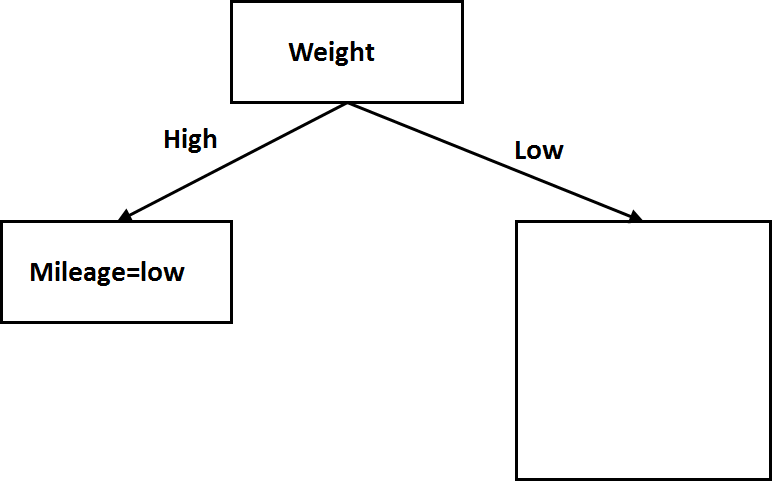
\includegraphics[scale=0.5]{dTreeEg1.png}
    \end{center}
\end{frame}
\begin{frame}{Building Decision Trees Intuition}
\begin{center}
    \begin{table}
        \begin{tabular}{| c | c | c |}
            \hline
            {\bf Horsepower} & {\bf Weight} & \textcolor{blue}{{\bf Mileage}} \\ \hline
                95 & low & low \\ \hline
                90 & low & low \\ \hline
                70 & low & high \\ \hline
                86 & low & high \\ \hline
        \end{tabular}
        \caption{Car Mileage Prediction from 1971}
    \end{table}
\end{center}
\end{frame}
\begin{frame}{Building Decision Trees Intuition}
    \begin{center}
        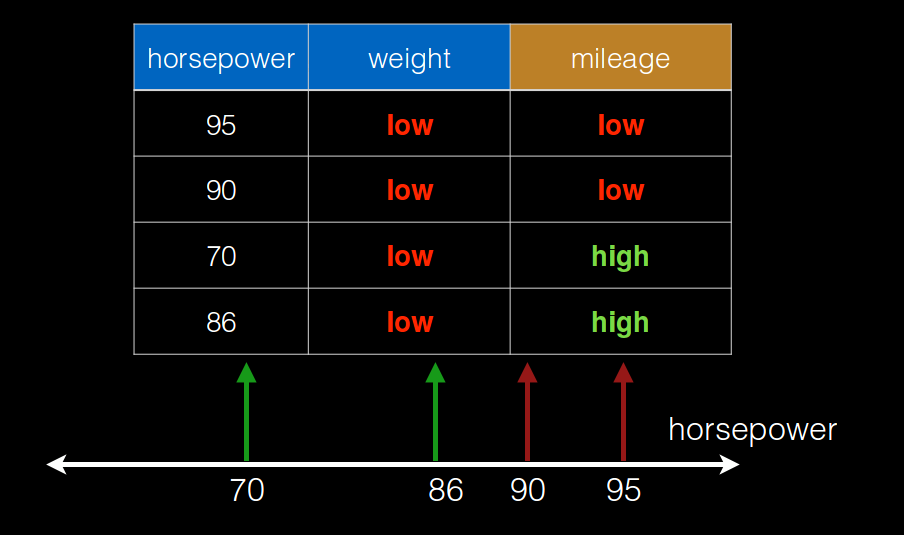
\includegraphics[scale=0.3]{dTreeEg2.png}
    \end{center}
\end{frame}
\begin{frame}{Building Decision Trees Intuition}
    \begin{center}
        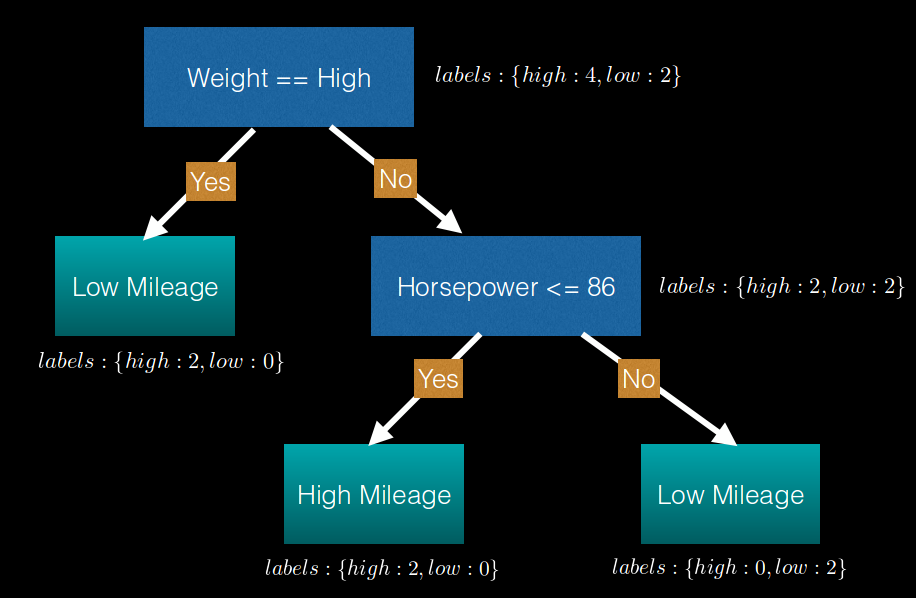
\includegraphics[scale=0.3]{dTreeEg3.png}
    \end{center}
\end{frame}
\begin{frame}{Building Decision Trees Intuition}

    {\bf Prediction:}
    \begin{center}
        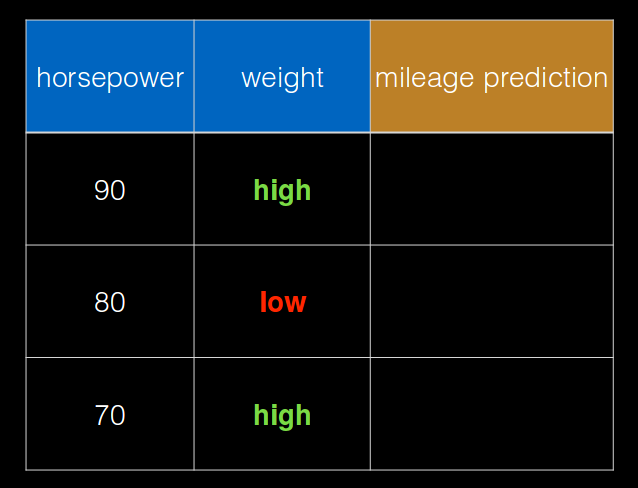
\includegraphics[scale=0.3]{dTreeEg4.png}
    \end{center}
\end{frame}
\begin{frame}{Building Decision Trees Intuition}

    {\bf Prediction:}
    \begin{center}
        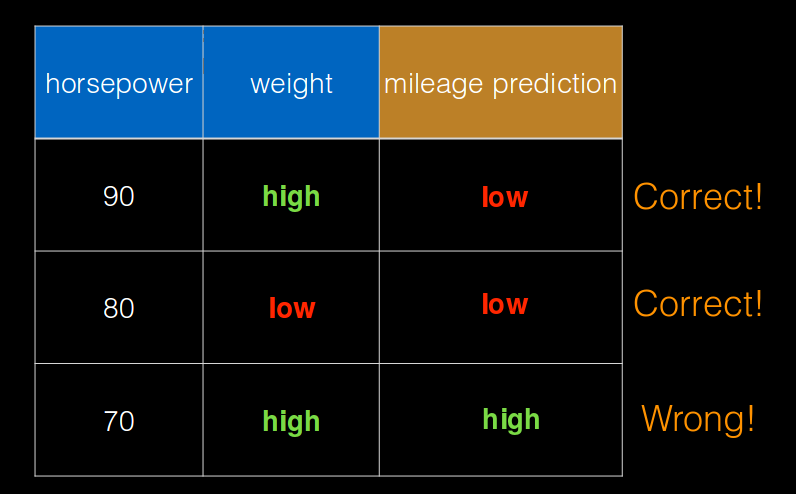
\includegraphics[scale=0.3]{dTreeEg5.png}
    \end{center}
\end{frame}


\section{Learning Decision Trees}
\begin{frame}{} 
    \begin{center}
        \thblue{Learning Decision Trees}
    \end{center}
\end{frame}

\begin{frame}{Decision Trees}
    \begin{itemize}
        \item Defined by a {\bf hierarchy} of rules (in form of a tree)
            \begin{center}
                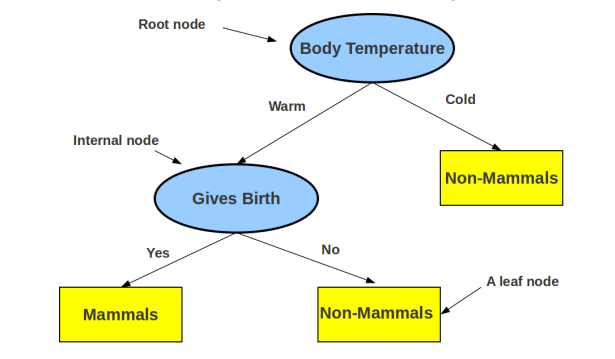
\includegraphics[scale=0.3]{dTreeExpl.png}
            \end{center}
        \item Rules form the internal nodes of the tree (topmost internal node = root)
        \item Each rule (internal node) tests the value of some property the data
        \item Leaf nodes make the prediction
    \end{itemize}
\end{frame}


\begin{frame}{Decision Tree Learning}

    {\bf Objective:} 
    \begin{itemize}
        \item Use the training data to construct a good decision tree
        \item Use the constructed Decision tree to predict labels for test inputs
    \end{itemize}
\end{frame}

\begin{frame}{Decision Tree Learning}
    \begin{itemize}
        \item Identifying the region (blue or green) a point lies in
        \begin{itemize}
            \item A classification problem (blue vs green)
            \item Each input has 2 features: co-ordinates $\{x_1, x_2\}$ in the 2D plane
        \end{itemize}
        \item Once learned, the decision tree can be used to predict the region (blue/green) of a new test point
    \end{itemize}
\end{frame}

\begin{frame}{Decision Tree Learning}
    \begin{center}
        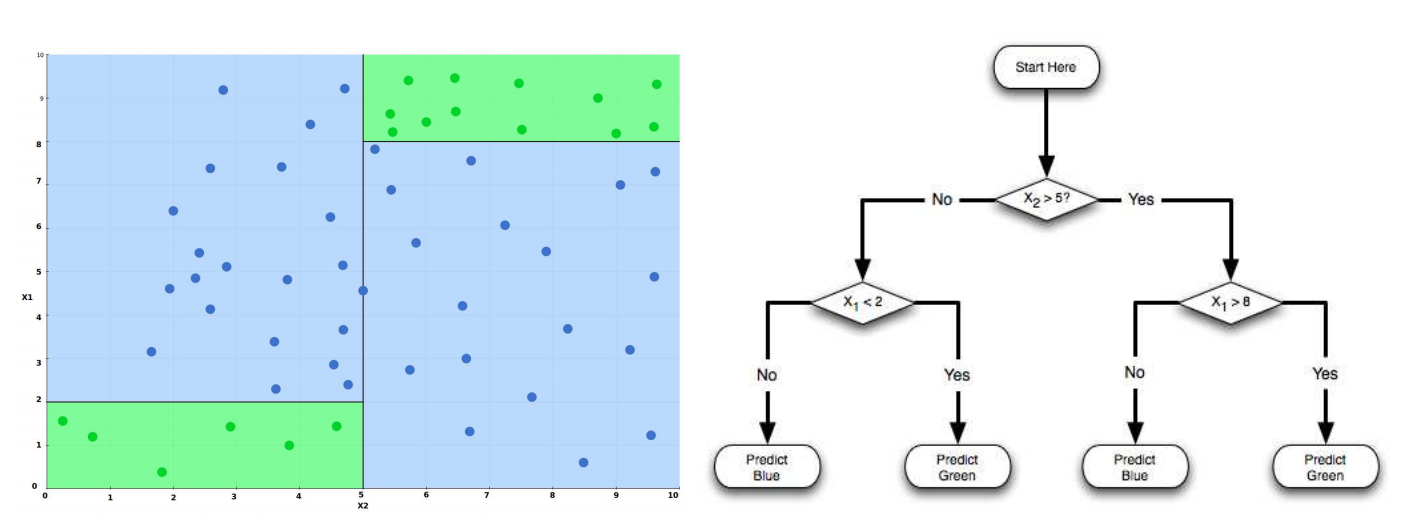
\includegraphics[scale=0.23]{dTreeLearning1.png}
    \end{center}
\end{frame}

\begin{frame}{Expressiveness of Decision Trees}
    \begin{columns}
        \column{0.48\linewidth}
            \centering
            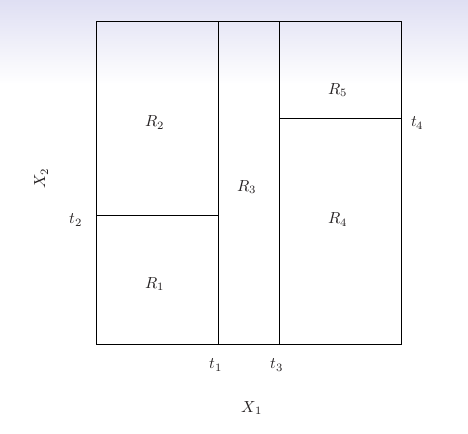
\includegraphics[scale=0.40]{dTreeExpressiveness1.png}
            
        \column{0.48\linewidth}
            \centering
            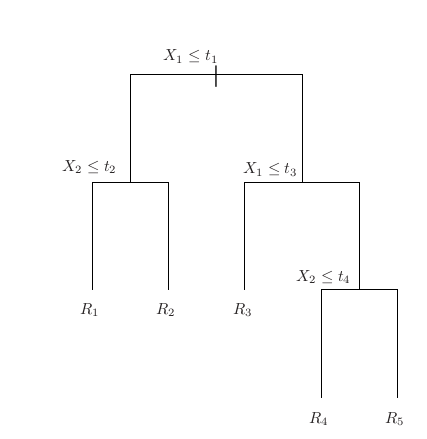
\includegraphics[scale=0.40]{dTreeExpressiveness2.png}
    \end{columns}
\end{frame}

\begin{frame}{Expressiveness of Decision Trees}
    \begin{itemize}
        \item Decision tree divides feature space into {\bf axis-parallel} rectangles
        \item Each rectangle is labelled with one of the $C$ classes
        \item Any partition of feature space by recursive binary splitting can be simulated by Decision Trees
    \end{itemize}
\end{frame}

\begin{frame}{Expressiveness of Decision Trees}
    \begin{columns}
        \column{0.48\linewidth}
            \centering
            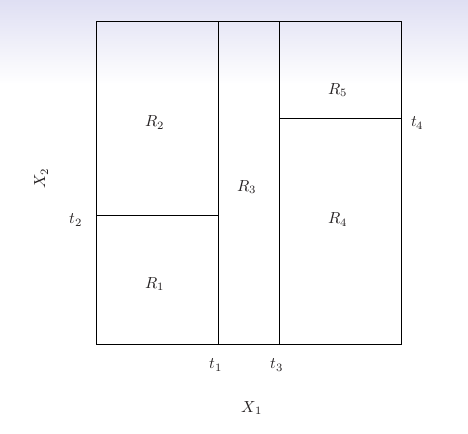
\includegraphics[scale=0.36]{dTreeExpressiveness1.png}
            
        \column{0.48\linewidth}
            \centering
            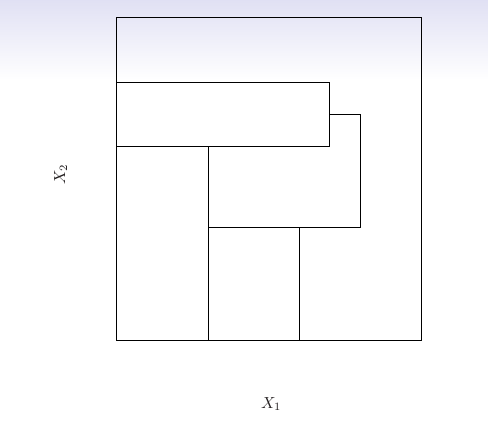
\includegraphics[scale=0.40]{dTreeExpressiveness3.png}
    \end{columns}

    \pause Feature space on left can be simulated by Decision tree but not the one on right.
\end{frame}

\begin{frame}{Expressiveness of Decision Tree}
    \begin{columns}
        \column{0.48\linewidth}
            \begin{itemize}
                \item Can express any logical function on input attributes
                \item Can express {\bf any} boolean function
                \item For boolean functions, path to leaf gives truth table row
                \item Could require exponentially many nodes
                \item $cyl=3 \vee (cyl=4 \wedge (maker=asia \vee maker=europe)) \vee \ldots $
            \end{itemize}
            
        \column{0.48\linewidth}
            \centering
            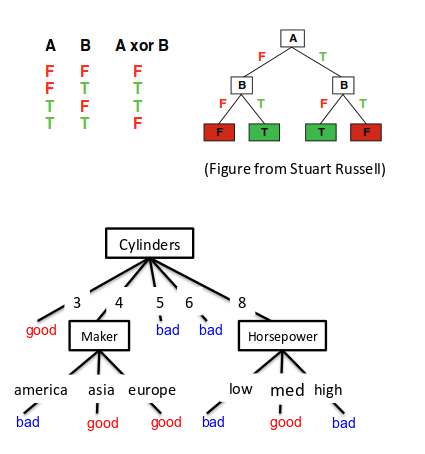
\includegraphics[scale=0.30]{dTreeFunctions.png}
    \end{columns}
\end{frame}

\begin{frame}{Hypothesis Space}
    \begin{itemize}
        \item Exponential search space wrt set of attributes
        \item If there are $d$ boolean attributes, then the search space has $2^{2^d}$ trees
        \begin{itemize}
            \item If $d=6$, then it is approximately $18,446,744,073,709,551,616$ (or approximately $1.8 \times 10^{18}$)
            \item If there are $d$ boolean attributes, each truth table has $2^d$ rows
            \item Hence there must be $2^{2^d}$ truth tables that can take all possible variations 
            \item Alternate argument: the number of trees is same as 
            \begin{itemize}
                \item number of bolean functions with $d$ variables
                \item = number of distinct truth tables with $2^d$ rows = $2^{2^d}$
            \end{itemize}
        \end{itemize}
        \item NP-Complete to find optimal decision tree
        \item Idea: Use greedy approach to find a locally optimal tree
    \end{itemize}
\end{frame}

\begin{frame}{Decision Tree Learning Algorithms}
    \begin{itemize}
        \item 1966: Hunt and colleagues from Psychology developed first known algorithm for human concept learning
        \item 1977: Breiman, Friedman and others from Statistics developed CART
        \item 1979: Quinlan developed proto-ID3
        \item 1986: Quinlan published ID3 paper
        \item 1993: Quinlan's updated algorithm C4.5
        \item 1980's and 90's: Improvements for handling noise, continuous attributes, missing data, non-axis parallel DTs, better heuristics for pruning, overfitting, combining DTs
    \end{itemize}
\end{frame}

\begin{frame}{Decision Tree Learning Algorithms}
    
    Main Loop:
    \begin{enumerate}
        \item Let $A$ be the ``best'' decision attribute for next node
        \item Assign $A$ as decision attribute for node
        \item For each value of $A$, create a new descendent of node
        \item Sort training examples to leaf nodes
        \item If training examples are perfectly classified, then STOP else iterate over leaf nodes
    \end{enumerate}
\end{frame}

\begin{frame}{Recursive Algorithm for Learning Decision Trees}
    \begin{center}
        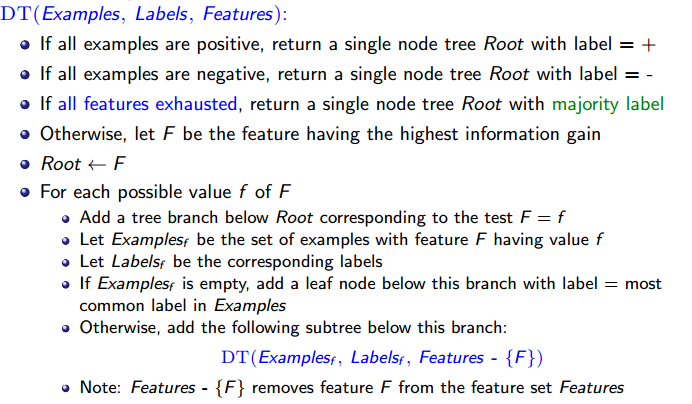
\includegraphics[scale=0.4]{dTreeLearningAlgo.png}
    \end{center}
\end{frame}


\begin{frame}{Decision Tree Learning}
    \begin{itemize}
        \item Greedy Approach: Build tree, top-down by choosing one attribute at a time
        \item Choices are locally optimal and may or may not be globally optimal 
        \item Major issues
        \begin{itemize}
            \item Selecting the next attribute
            \item Given an attribute, how to specify the split condition
            \item Determining termination condition
        \end{itemize}
    \end{itemize}
\end{frame}

\begin{frame}{Termination Condition}

    Stop expanding a node further when: \pause
    \begin{itemize}
        \item It consist of examples all having the same label 
        \item Or we run out of features to test!
    \end{itemize}
\end{frame}


\begin{frame}{How to Specify Test Condition?}
    \begin{itemize}
        \item Depends on attribute types
        \begin{itemize}
            \item Nominal
            \item Ordinal
            \item Continuous
        \end{itemize}
        \item Depends on number of ways to split
        \begin{itemize}
            \item 2-way split
            \item Multi-way split
        \end{itemize}
    \end{itemize}
\end{frame}


\begin{frame}{Splitting based on Nominal Attributes}
    \begin{center}
        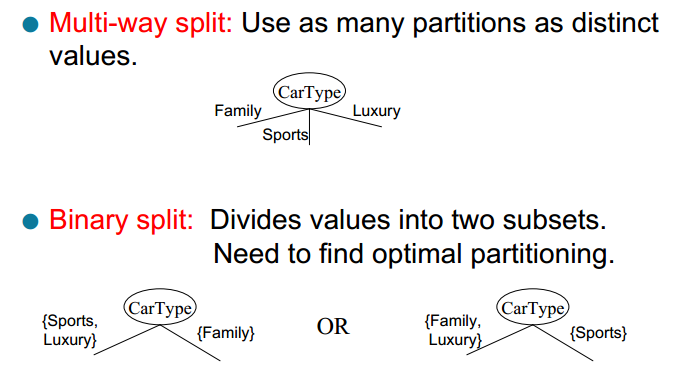
\includegraphics[scale=0.4]{splittingNominalAttr.png}
    \end{center}
\end{frame}
\begin{frame}{Splitting based on Ordinal Attributes}
    \begin{center}
        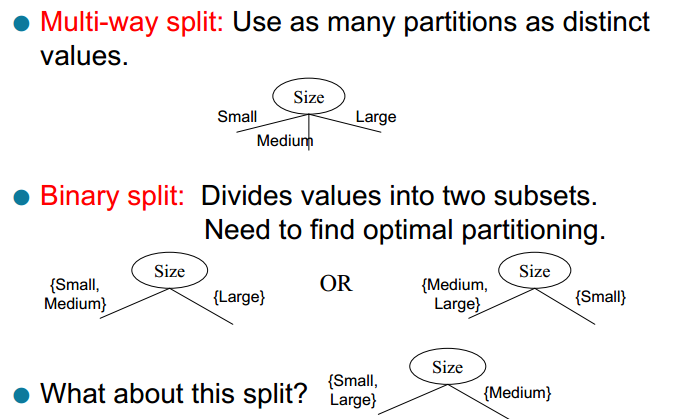
\includegraphics[scale=0.4]{splittingOrdinalAttr.png}
    \end{center}
\end{frame}
\begin{frame}{Splitting based on Continuous Attributes}

    How to split continuous attributes such as Age, Income etc
    \pause 
    \begin{itemize}
        \item {\bf Discretization} to form an ordinal categorical attribute
        \begin{itemize}
            \item {\em Static:} discretize once at the beginning
            \item {\em Dynamic:} find ranges by equal interval bucketing, equal frequency bucketing, percentiles, clustering etc
        \end{itemize}
        \item {\bf Binary Decision:} $ (A < v) or (A \geq v)$
        \begin{itemize}
            \item Consider all possible split and find the best cut
            \item Often, computationally intensive
        \end{itemize}
    \end{itemize}
\end{frame}
\begin{frame}{Splitting based on Continuous Attributes}
    \begin{center}
        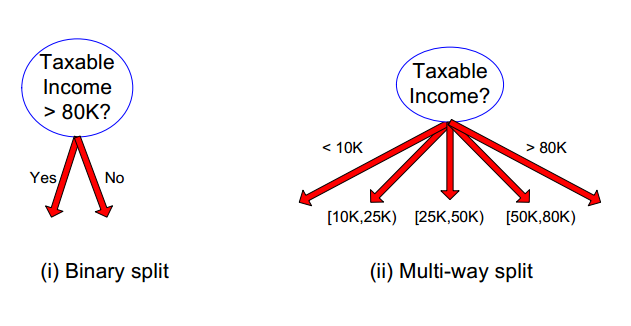
\includegraphics[scale=0.5]{splittingContAttr.png}
    \end{center}
\end{frame}

\begin{frame}{Choosing the next Attribute - I}
    \begin{center}
        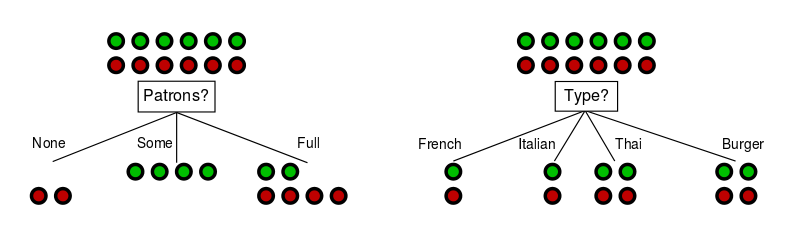
\includegraphics[scale=0.4]{choosingNextAttr1.png}
    \end{center}
\end{frame}
\begin{frame}{Choosing the next Attribute - II\furl{http://www.cedar.buffalo.edu/~srihari/CSE574/Chap16/Chap16.1-InformationGain.pdf}}
    \begin{center}
        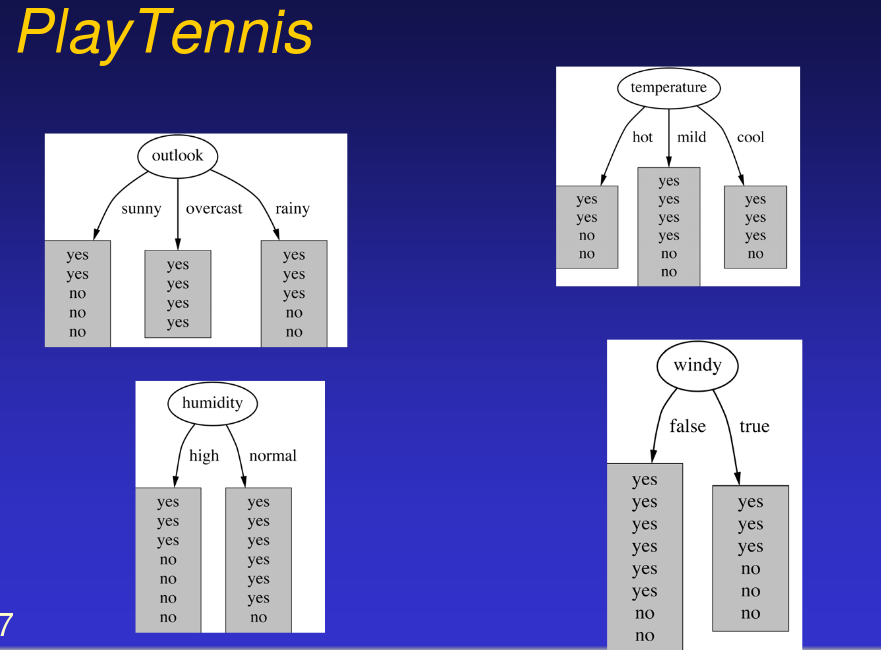
\includegraphics[scale=0.3]{choosingNextAttr2.png}
    \end{center}
\end{frame}
\begin{frame}{Choosing the next Attribute - III}
    \begin{center}
        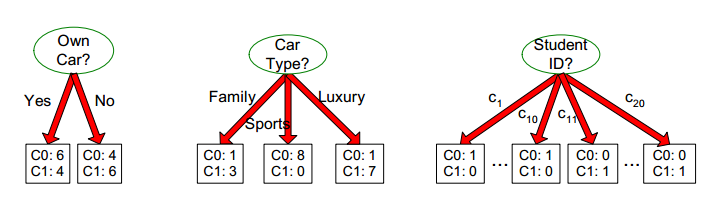
\includegraphics[scale=0.45]{choosingNextAttr3.png}
    \end{center}
\end{frame}

\begin{frame}{Choosing an Attribute}
    \begin{itemize}
        \item Good Attribute \pause
        \begin{itemize}
            \item for one value we get all instances as positive
            \item for other value we get all instances as negative
        \end{itemize}
        \item Bad Attribute \pause
        \begin{itemize}
            \item it provides no discrimination
            \item attribute is immaterial to the decision
            \item for each value we have same number of positive and negative instances
        \end{itemize}
    \end{itemize}
\end{frame}


\begin{frame}{How to Find the Best Split?}
    \begin{center}
        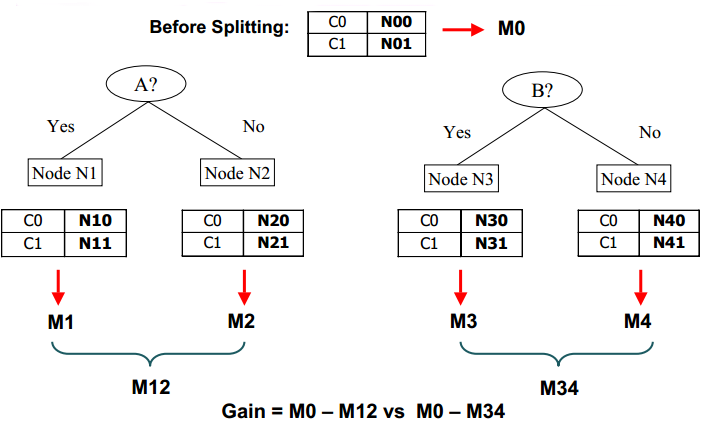
\includegraphics[scale=0.4]{howToFindBestSplit.png}
    \end{center}
\end{frame}


\begin{frame}{Measures of Node Impurity}
    \begin{itemize}
        \item Gini Index
        \item Entropy
        \item Misclassification Error
    \end{itemize}
\end{frame}


\begin{frame}{Gini Index}
    \begin{itemize}
        \item An important measure of statistical dispersion
        \item Used in Economics to measure income inequality in countries
        \item Proposed by Corrado Gini 
    \end{itemize}
\end{frame}
\begin{frame}{Gini Index}
    \begin{center}
        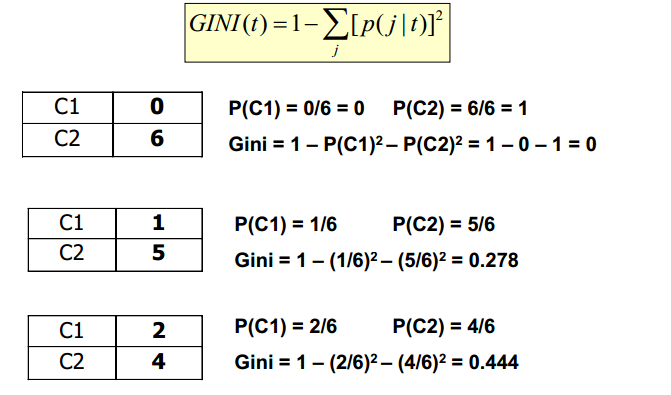
\includegraphics[scale=0.4]{giniIndex2.png}
    \end{center}
\end{frame}
\begin{frame}{Gini Index}
    \begin{center}
        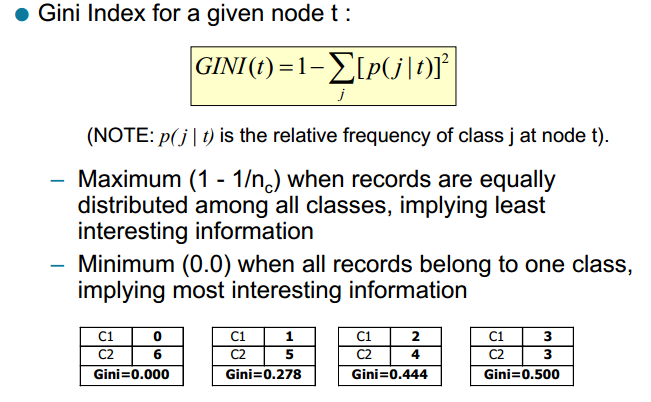
\includegraphics[scale=0.4]{giniIndex1.png}
    \end{center}
\end{frame}
\begin{frame}{Splitting Based on Gini}
    \begin{itemize}
        \item Used in CART, SLIQ, SPRINT
        \item When a node $p$ is split into $k$ partitions (children), the quality of split is computed as,
                $$ Gini_{split} = \sum_{i=1}^{k} \frac{n_i}{n} Gini(i) $$
        \begin{itemize}
            \item $n_i$ =  number of records at child $i$
            \item $n$ =  number of records at node $p$
        \end{itemize}
    \end{itemize}
\end{frame}
\begin{frame}{Gini Index for Binary Attributes}
    \begin{center}
        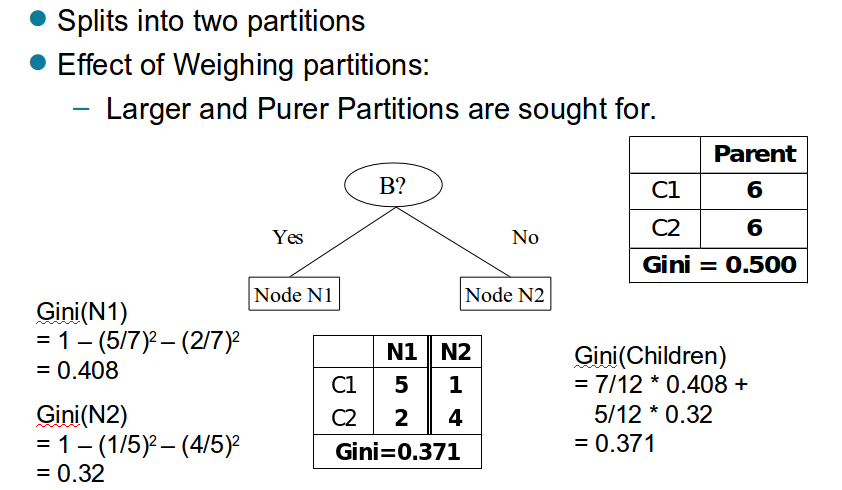
\includegraphics[scale=0.4]{giniIndex3.png}
    \end{center}
\end{frame}
\begin{frame}{Gini Index for Categorical Attributes}
    \begin{center}
        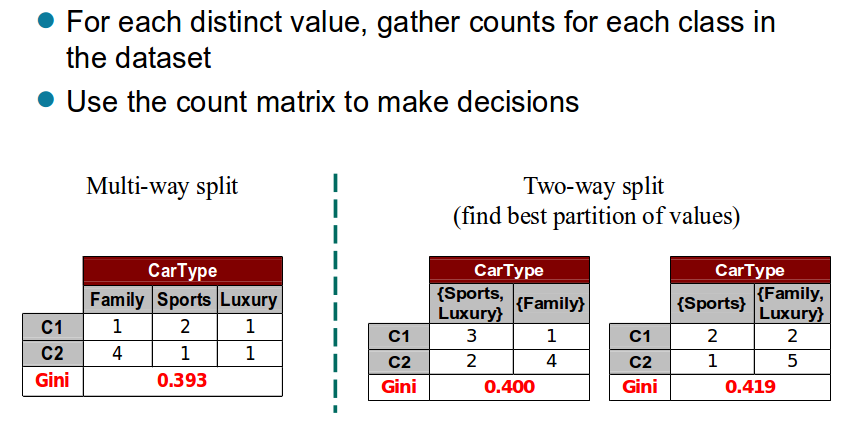
\includegraphics[scale=0.4]{giniIndex4.png}
    \end{center}
\end{frame}

\begin{frame}{Entropy and Information Gain}
    \begin{itemize}
        \item You are watching a set of independent random samples of a random variable $X$
        \item Suppose the probabilities are equal: $P(X=A) = P(X=B) = P(X=C) = P(X=D) = \frac{1}{4}$
        \item Suppose you see a text like $BAAC$
        \item You want to transmit this information in a {\bf binary} communication channel
        \item How many bits will you need to transmit this information? \pause
        \item Simple idea: Represent each character via 2 bits: $A=00, B=01, C=10, D=11$
        \item So, $BAAC$ becomes $01000010$
        \item Communication Complexity: $2$ on average bits per symbol
    \end{itemize}
\end{frame}

\begin{frame}{Entropy and Information Gain}
    \begin{itemize}
        \item Suppose you knew probabilities are unequal: $P(X=A) = \frac{1}{2}, P(X=B) = \frac{1}{4}, P(X=C) = P(X=D) = \frac{1}{8}$
        \item It is now possible to send information $1.75$ bits on average per symbol \pause
        \item Choose a frequency based code!
        \item $A=0, B=10, C=110, D=111$ \pause
        \item $BAAC$ becomes $1000110$
        \item Requires only 7 bits for transmitting $BAAC$
    \end{itemize}
\end{frame}

\begin{frame}{Entropy}
    \begin{center}
        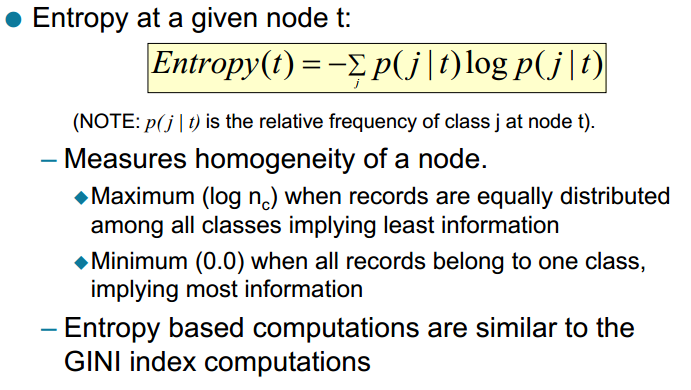
\includegraphics[scale=0.4]{entropy1.png}
    \end{center}
\end{frame}
\begin{frame}{Entropy}
    \begin{center}
        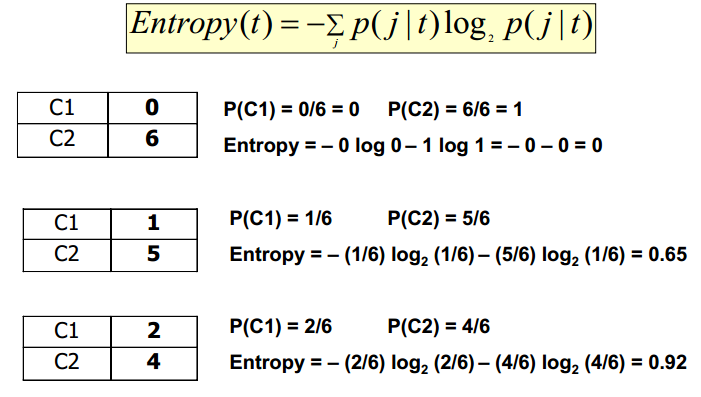
\includegraphics[scale=0.4]{entropy2.png}
    \end{center}
\end{frame}
\begin{frame}{Entropy}
    \begin{center}
        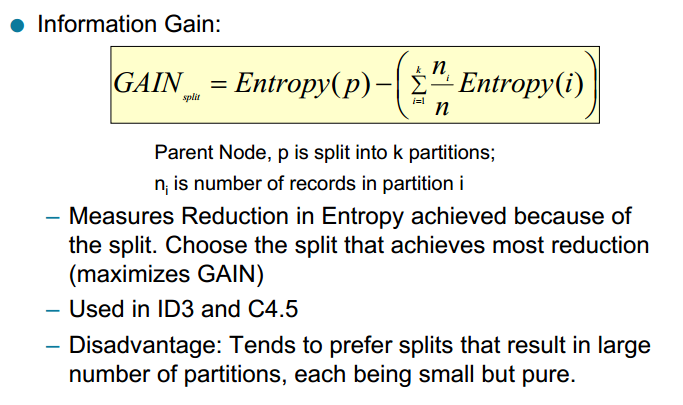
\includegraphics[scale=0.4]{entropy3.png}
    \end{center}
\end{frame}
\begin{frame}{Entropy}
    \begin{center}
        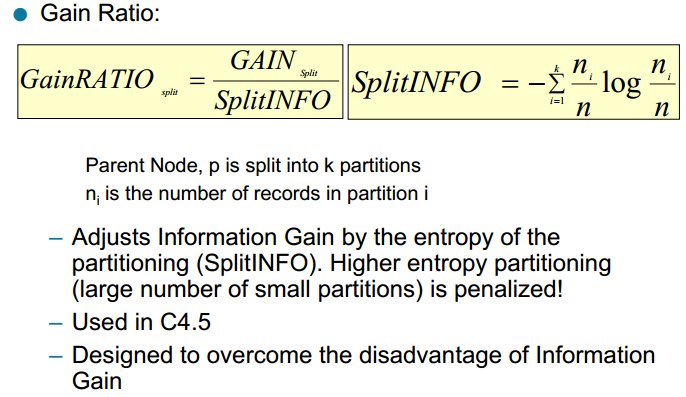
\includegraphics[scale=0.4]{entropy4.png}
    \end{center}
\end{frame}


\begin{frame}{Splitting based on Classification Error}
    \begin{itemize}
        \item Classification error at node $t$ is $$Error(t) = 1 - max_{i} P(i|t)$$
        \item Measures misclassification error made by a node.
        \begin{itemize}
            \item Minimum ($0.0$) when all records belong to one class, implying  most interesting information
            \item Maximum ($1 - \frac{1}{n_c}$) when records are equally distributed among all classes, implying least interesting information
        \end{itemize}
    \end{itemize}
\end{frame}
\begin{frame}{Classification Error}
    \begin{center}
        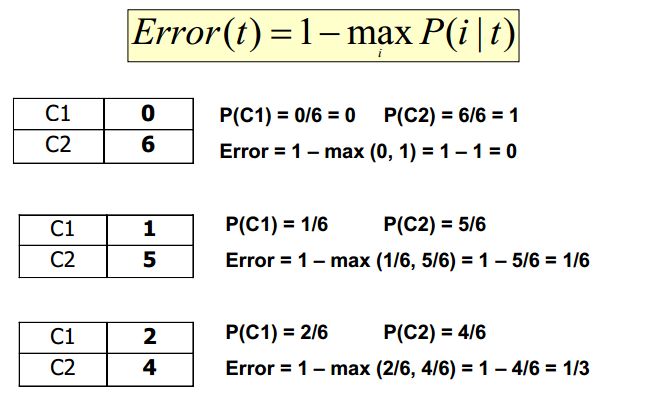
\includegraphics[scale=0.4]{classificationError.png}
    \end{center}
\end{frame}

\begin{frame}{Comparison among Splitting Criteria}
    \begin{center}
        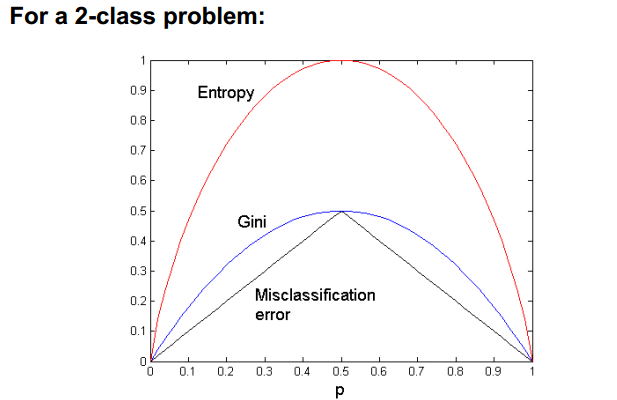
\includegraphics[scale=0.4]{comparingSplittingCritieria.png}
    \end{center}
\end{frame}
\begin{frame}{Splitting Criteria}
    \begin{itemize}
        \item Gini Index (CART, SLIQ, SPRINT):
        \begin{itemize} 
            \item select attribute that minimize impurity of a split 
        \end{itemize}
        \item Information Gain (ID3, C4.5)
        \begin{itemize} 
            \item select attribute with largest information gain
        \end{itemize}
        \item Normalized Gain ratio (C4.5)
        \begin{itemize} 
            \item normalize different domains of attributes
        \end{itemize}
        \item  Distance normalized measures (Lopez de Mantaras)
        \begin{itemize} 
            \item define a distance metric between partitions of the data
            \item chose the one closest to the perfect partition
        \end{itemize}
        \item $\chi^2$ contingency table statistics (CHAID)
        \begin{itemize} 
            \item measures correlation between each attribute and the class label
            \item select attribute with maximal correlation
        \end{itemize}
    \end{itemize}
\end{frame}

\begin{frame}{Overfitting in Decision Trees}
    \begin{itemize}
        \item Decision trees will always overfit in the absence of label noise
        \item Simple strategies for fixing:
        \begin{itemize}
            \item Fixed depth
            \item Fixed number of leaves
            \item Grow the tree till the gain is above some threshold
            \item Post pruning
        \end{itemize}
    \end{itemize}
\end{frame}

\begin{frame}{Trees vs Linear Models}
    \begin{center}
        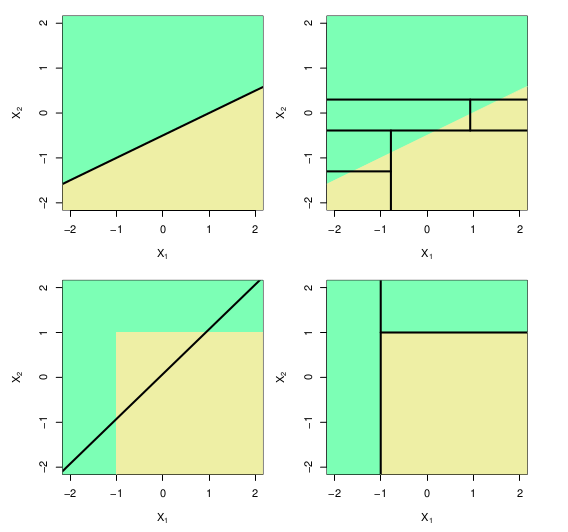
\includegraphics[scale=0.4]{treesVsLinearModels.png}
    \end{center}
\end{frame}

\begin{frame}{Advantages and Disadvantages}
    \begin{itemize}
        \item Very easy to explain to people.
        \item Some people believe that decision trees more closely mirror human decision-making
        \item Trees can be displayed graphically, and are easily interpreted even by a non-expert (especially if they are small)
        \item Trees can easily handle qualitative predictors without the need to create dummy variables.
        \item Inexpensive to construct
        \item Extremely fast at classifying new data
        \item Unfortunately, trees generally do not have the same level of predictive accuracy as other classifiers
    \end{itemize}
\end{frame}


\section{Summary}
\begin{frame}{Summary}

\tblue{Major Concepts:}
\begin{itemize}
    \item Geometric interpretation of Classification
    \item Decision trees
\end{itemize}
\end{frame}

\begin{frame}{Slide Material References}
\begin{itemize}
    \item Slides from ISLR book
    \item Slides by Piyush Rai
    \item Slides for Chapter 4 from ``Introduction to Data Mining'' book by Tan, Steinbach, Kumar
    \item Slides from Andrew Moore, CMU
    \item See also the footnotes
\end{itemize}
\end{frame}


\end{document}

